\chapter{Advantages and Applications}
\section{Advantages}


\begin{minipage}[c]{0.45\textwidth}
\begin{enumerate}
    \item Cost effective : Compared with available AGVs in the market, this AGV costs much less
    \item Small and compact : As AGV is small is size so can be used in small scale industries as well.
    \item Close-to-market : AGV meets the current market needs and we can directly implement it by scaling to the required extent.
    \item Remote control : AGV can be controlled wireless from the remote place using the GUI.
\end{enumerate}
\end{minipage}
\hfill
\begin{minipage}[c]{0.4\textwidth}
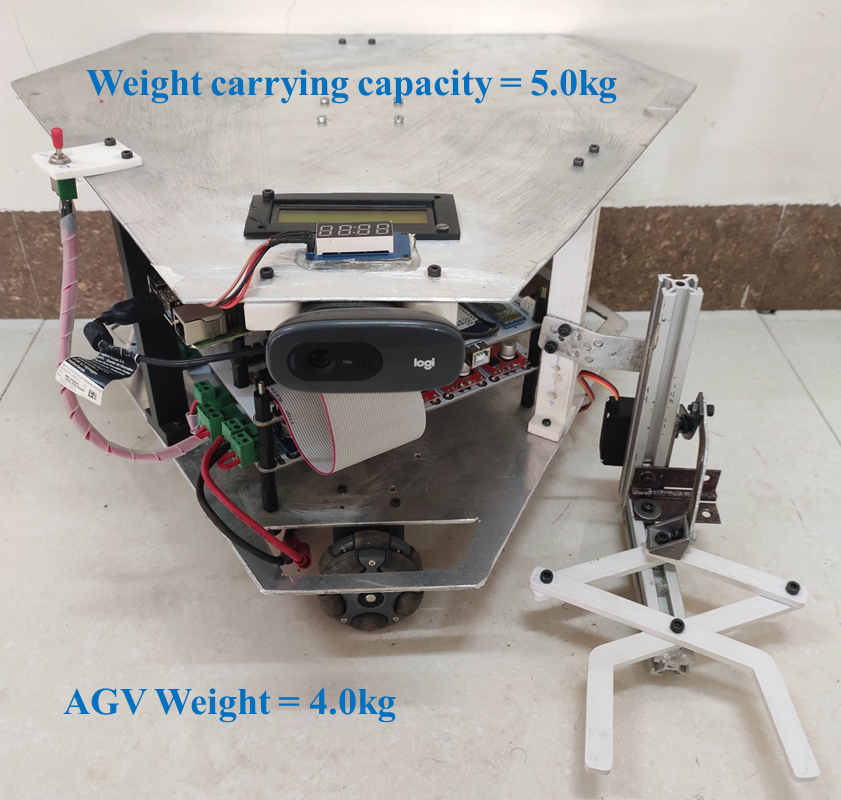
\includegraphics[width=\textwidth]{project/images/agv03.png}
\end{minipage}
\begin{enumerate}
    \setItemnumber{4}
    \item Multi-Tasking : With the help of multiple techniques implemented in AGV, it can be multiple tasks and will be helpful in increasing the productivity.
    \item Semi-autonomous : AGV can be controlled manually as well as it can operate automatically. Thus it is said to be semi-autonomous.
    \item Cutting-edge technology : The AGV is developed using cutting edge technologies like Computer Vision, Machine Learning, etc.
    \item Reduced labor costs : Using AGVs in the warehouses can help in replacing them instead of labors working there. Thus it reduces the labor cost of the industry.
    \item Increased accuracy and productivity : Automation in industry decreases the random and human errors, and results in increased accuracy and productivity of work.
    %\item High availability/reliability
    % \item Integrated operation of all AGVs
    % \item Random material handling capability due to programmability
\end{enumerate}

\newpage
\section{Applications}
\begin{enumerate}
    \item Manufacturing : AGVs are used in manufacturing units for carrying parts from one location to another.
    \item Chemical :
    \item Pharmaceutical
    \item Paper and print
    \item Food and beverage : Packing, delivering of beverage bottles,food packets can be done using the AGVs in food and beverage industries. 
    \item Hospital : Well equipped AGVs in the hospitals can be used to assist the doctor in the operation theatres, to serve food to patients in the wards, etc. These can be the most useful solution after the post COVID-19 pandemic situation for the hospitals.
    \item Warehousing : Similar to the manufacturing industry, in warehouses also, AGVs can be used to transport objects from one location to another, from loading zones to dispatching areas.
    \item Theme Parks
\end{enumerate}

